\section{Bumblebeets mit Brokkolieis}
\begin{tikzpicture}[remember picture,overlay]
    \node[anchor=east,yshift=-4cm,inner sep=0pt] at (current page text area.east|-0,3cm) {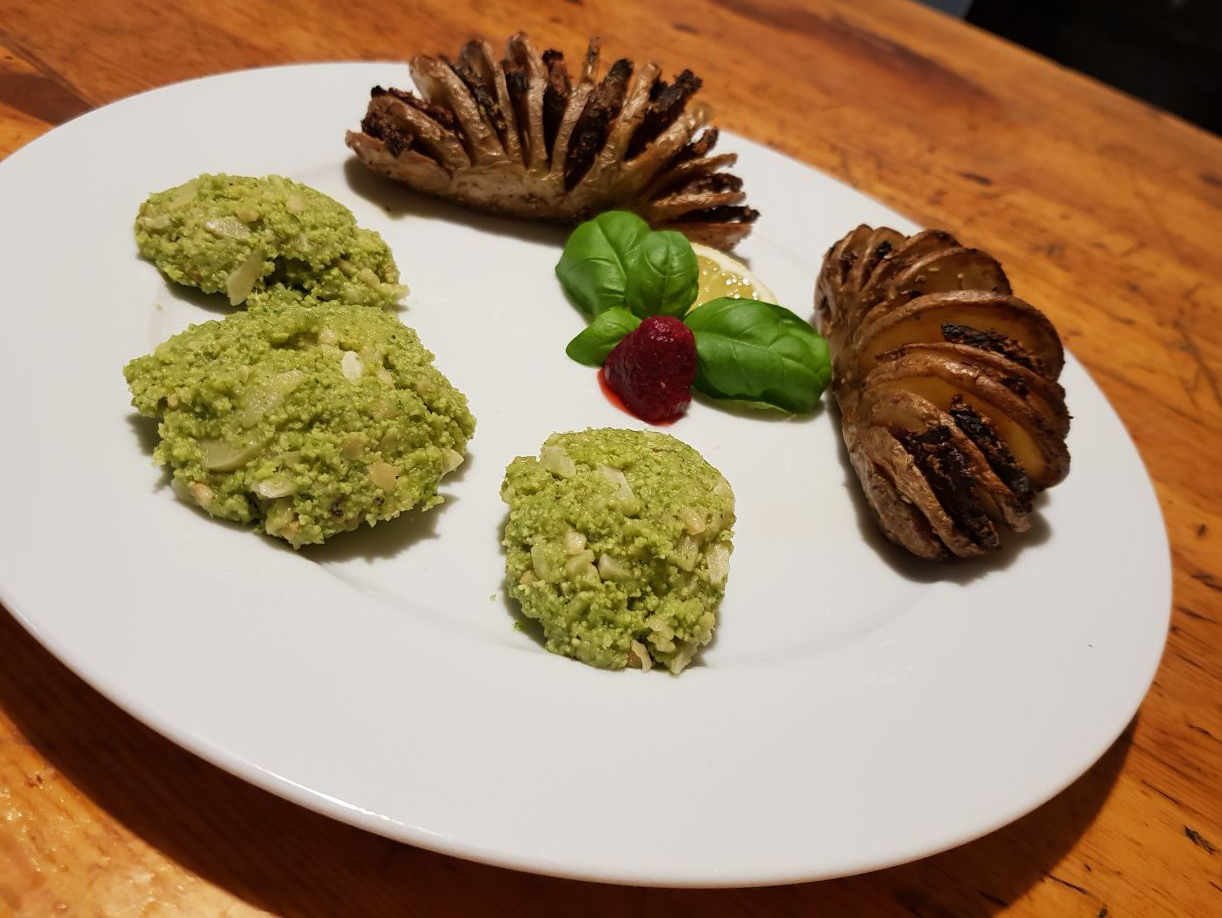
\includegraphics[height=5cm]{/Users/dertoast/Documents/Zeug/Küche/Munchies/res/bumblebeets.png}};
\end{tikzpicture}
\subsection*{Brokkoli-Eiscreme}\label{subsec:broc-icecream}
\subsubsection*{Eismasse}
\begin{longtable}{rlL{15,8cm}}
    200g                    &   Brokkoli        &   kurz in    \\
    100g                    &   Butter\footnote{gerne auch vegan z.B. \href{https://www.bio123.de/produkt/naturli/naturli-organic-vegan-block-200g}{Naturli vegan block}
									        oder \href{https://www.alsan.de/alsan-bio/}{Alsan}}
                                                &   dünsten.
                                                    Dann mit    \\
    100ml                   &   Haselnussmilch  &   ablöschen und   \\
    $\frac{1}{2}$TL (4g)    &   Salz            &   sowie \\
    20ml                    &   Weißwein        &   zugeben und pürieren    \\
\end{longtable}
\subsubsection*{Frieren}
\emph{Die Frierzeiten sind abhängig von Menge und Gefrierfach/-schrank.}
\begin{longtable}{rlL{14,6cm}}
    Ca. $\frac{3}{4}$ Std.  &   im Gefrierfach                  &   anfrieren lassen.   \\
    Ca. 1 Std.              &   weiter frieren                  &   , dabei aber \mins{alle 20} mit einem Schneebesen verquirlen \\
    \textbf{50g}            &   \textbf{Mandelstifte}           &   und \\
    \textbf{50g}            &   \textbf{gehackte Haselnüsse}    &   unterrühren und dann weitere    \\
    1 Std.                  &   frieren                         &   und dabei \mins{alle 20} mit einem Teigschaber umrühren. \\
\end{longtable}

\subsection*{Kartoffel-Rote Beete-Fächer}\label{subsec:bumblebeets}
Die Gewürz-Öl Mischungen sollten zuerst zubereitet werden, damit die Aromen besser durchziehen können.
\subsubsection*{Rote Beete}\label{subsubsec:beets}
\begin{longtable}{rlL{16.9cm}}
    1 TL            &   Kreuzkümmel &   zusammen mit    \\
    2 TL            &   Senfkörnern &   mörsern. Von    \\
    $\frac{1}{2}$   &   Zitrone     &   Zesten reißen und fein hacken.  \\
    3 EL            &   Olivenöl    &   und gemöserte Gewürze damit zu einer Würzpaste vermischen.  \\
    2               &   rote Beeten &   in 3mm dicke Scheiben schneiden und mit Würpaste bestreichen.\\
\end{longtable}

\subsubsection*{Kartoffeln}
Ofen auf \cel{200} vorheizen
\begin{longtable}{rlL{16.8cm}}
    3       &   Knoblauchzehen      &   und \\
            &   Rosmarin            &   möglichst fein schneiden und mit    \\
    7 EL    &   Olivenöl            &   zu einem Würzöl vermischen. \\
    4       &   große Kartoffeln    &   scheibenartig (ca. 7mm) einschneiden (nicht ganz durch, sie sollen später aufgefächert werden). \\
\end{longtable}
Die Kartoffeln mit Würzöl bestreichen und für \mins{20} vorbacken, bis man sie auffächern kann, ohne sie dabei zu zerbrechen.
Dann die gewürzten \nameref{subsubsec:beets}-Scheiben in die Lücken stecken und weitere \mins{20-30} backen.

Die fertigen \nameref{subsec:bumblebeets} mit je einer Kugel \nameref{subsec:broc-icecream} und einem Schnitz Zitrone servieren.
Zur Dekoration eignen sich Basilikumblätter und Himbeeren, da beides geschmacklich auch sehr gut passt.
